\documentclass{beamer}

\usepackage[utf8]{inputenc}
\usepackage{fancyvrb}
\usepackage{color}
\usepackage[export]{adjustbox}
\usepackage{ulem}

\include{pygments_java}
\include{pygments_props}

\usetheme{Antibes}
\usecolortheme{seahorse}

\useoutertheme{infolines}
\setbeamertemplate{blocks}[default]
\setbeamertemplate{items}[triangle]
\setbeamertemplate{enumerate items}[square]
\setbeamertemplate{sections/subsections in toc}[square]
\setbeamertemplate{navigation symbols}{}

\setbeamerfont{code}{size*={8}{10}}

\newcommand{\bigtextframe}[1]{
  \begin{frame}
    \begin{beamercolorbox}[center]{note}
      \Huge #1
    \end{beamercolorbox}
  \end{frame}
}

\newcommand{\diagram}[2][1]{
  \begin{center}
    \includegraphics[height=0.7\paperheight,width=#1\paperwidth,keepaspectratio]{#2}
  \end{center}
}

\newlength{\wideitemsep}
\setlength{\wideitemsep}{\itemsep}
\addtolength{\wideitemsep}{5pt}
\let\olditem\item
\renewcommand{\item}{\setlength{\itemsep}{\wideitemsep}\olditem}

\AtBeginSubsection[]
{
  \begin{frame}{Outline}
    \tableofcontents[sectionstyle=show/shaded,subsectionstyle=show/shaded/hide]
  \end{frame}
}

\title{Fetch from follower can save you oodles}
\subtitle{Real world impact of implementing KIP-392 in a cloud environment}
\author[Jan Urbański]{Jan Urbański \\ \texttt{jan@newrelic.com}}
\institute{New Relic}
\date[Kafka Summit 2024]{Kafka Summit 2024, London, March 19-20}

\begin{document}


\frame{\titlepage}

\begin{frame}[fragile]
  \frametitle{For those following at home}

  \begin{block}{Getting the slides}
    \begin{semiverbatim}
    \$ wget https://wulczer.org/fetch-from-follower.pdf
    \end{semiverbatim}
  \end{block}

  \begin{block}{Getting the source}
    \begin{semiverbatim}
    \$ wget https://github.com/wulczer/fetch-from-follower
    \end{semiverbatim}
  \end{block}
\end{frame}

\begin{frame}
  \tableofcontents
\end{frame}

\section{What is fetch from follower}
\subsection{Overview of the functionality}

\begin{frame}
  \frametitle{What is fetch from follower}

  \begin{itemize}
  \item a fetch protocol extension that allows consumers to \alert{fetch from replicas}
    \begin{itemize}
    \item also known as \alert{KIP-392}
    \item available from \alert{Kafka 2.4.0}
    \end{itemize}
  \item \alert{transparent} for consumers and backwards compatible
    \begin{itemize}
      \item also means it can be safely toggled on and off
    \end{itemize}
  \item controlled by the \alert{broker}, but needs extra information from the \alert{client}
  \end{itemize}
\end{frame}

\begin{frame}
  \frametitle{The general idea}

  \begin{itemize}
  \item an in-sync follower for a partition will \alert{typically} have the data requested by the customer
  \item in a RF=3 system running in three racks, the brokers in each rack have \alert{all the data} from \alert{all partitions}
  \item \alert{all} consumer fetches can be done to a broker in the \alert{same rack}
  \end{itemize}
\end{frame}

\begin{frame}
  \frametitle{Determining the right broker}

  \begin{itemize}
  \item fetch requests could \alert{already} be sent to any broker
  \item brokers \alert{already} supported \texttt{broker.rack} to denote placement
  \item instead of letting clients choose which broker to fetch from, the \alert{broker returns a \textit{preferred read replica}} from fetch responses
    \begin{itemize}
    \item this means that the \alert{first} fetch request will always go to the \alert{leader}
    \item clients \alert{cache} preferred replicas for \texttt{metadata.max.age.ms} and then \alert{re-request} from the leader
    \end{itemize}
  \item all the client needs to do is set \alert{\texttt{client.rack}} on the fetch request
  \end{itemize}
\end{frame}

\begin{frame}
  \frametitle{Fetch flow}

  \diagram{fetch-flow}
\end{frame}

\subsection{Implementation details}

\begin{frame}
  \frametitle{Client changes}

  \begin{itemize}
  \item add a \alert{new config parameter} called \texttt{client.rack}
  \item include its value in \alert{fetch requests}
  \item look for a \alert{preferred replica ID} in fetch responses and cache it
  \item if we have a preferred replica for a partition, \alert{fetch from that} instead of the leader
  \item revert back to \alert{fetching from leader} if \texttt{OFFSET\_OUT\_OF\_RANGE} is received
  \end{itemize}
\end{frame}

\begin{frame}
  \frametitle{Broker changes}

  \begin{itemize}
  \item determine \alert{preferred replica} when handling fetch requests
    \begin{itemize}
    \item only \alert{partition leaders} will return preferred replicas
    \item \alert{pluggable} selector interface to compute the preferred replica
    \item \alert{built-in} rack-aware replica selector class
    \end{itemize}
  \item handle \alert{edge cases} like when the consumer tries fetching a committed offset that's not available on the replica
    \begin{itemize}
    \item the KIP itself has a good explanation of the new edge scenarios
    \end{itemize}
  \end{itemize}
\end{frame}

\begin{frame}
  \frametitle{Replica selection}

  \begin{beamercolorbox}[sep=1em]{code}
    \usebeamerfont{code}
    \include{ReplicaSelector}
  \end{beamercolorbox}
\end{frame}

\subsection{Why even bother?}

\begin{frame}
  \frametitle{Why bother?}

  \begin{itemize}
  \item \alert{cloud deployments} of Kafka clusters commonly span datacenters
    \begin{itemize}
    \item for example, MSK forces you to have replicas in \alert{each AZ}
    \end{itemize}
  \item partitions are \alert{evenly distributed} among AZs
  \item for a three-AZ deployment, around 2/3 of the fetches are \alert{cross-AZ}... \uncover<2>{which costs \alert{money}}
  \end{itemize}
\end{frame}

\usebackgroundtemplate{
  
\includegraphics[keepaspectratio,width=\paperwidth]{money.png}
}

\begin{frame}[plain]
\end{frame}
\usebackgroundtemplate{}

\begin{frame}
  \frametitle<1>{Without KIP-392}
  \frametitle<2>{Without KIP-392 - money!}
  \frametitle<3>{With KIP-392 - it's all free!}

  \only<1>{\diagram{cross-az-fetch-1}}
  \only<2>{\diagram{cross-az-fetch-2}}
  \only<3>{\diagram{cross-az-fetch-3}}
\end{frame}

\section{Configuring your cluster for KIP-392}
\subsection{Configuration properties}

\begin{frame}
  \frametitle{Broker properties}

  \begin{beamercolorbox}[sep=1em]{code}
    \usebeamerfont{code}
    \include{broker}
  \end{beamercolorbox}

  \uncover<2>{\huge{That's it!}}
\end{frame}

\begin{frame}
  \frametitle{Consumer properties}

  \begin{beamercolorbox}[sep=1em]{code}
    \usebeamerfont{code}
    \include{consumer}
  \end{beamercolorbox}

  \uncover<2>{\huge{That's it!}}
\end{frame}

\begin{frame}
  \frametitle{Easier said than done}

  \begin{itemize}
  \item configuring \alert{brokers} is relatively easy
    \begin{itemize}
    \item MSK even does that for you by default
    \end{itemize}
  \item configuring \alert{clients} depends on how much control you have
    \begin{itemize}
    \item New Relic has more than \alert{oe hundred} Kafka consumers
    \item fortunately, they all use a \alert{common startup script}
    \end{itemize}
  \item query the AWS \alert{meta endpoint} on startup for placement info
  \item use the AZ as \alert{\texttt{client.rack}}
  \end{itemize}
\end{frame}

\subsection{Verification}

\begin{frame}
  \frametitle{How do I know it worked?}

  \begin{itemize}
  \item a \alert{JMX metric} \texttt{preferred-read-replica} in the \texttt{consumer-fetch-manager-metrics} group reports the preferred replica ID
  \item the metric is recorded per client, topic, and partition
  \item but really, it's better to just look at the \alert{money}
  \end{itemize}
\end{frame}

\section{Show me the money}
\subsection{Results of rolling out KIP-392}

\begin{frame}
  \frametitle{We push some traffic}

  \begin{center}
    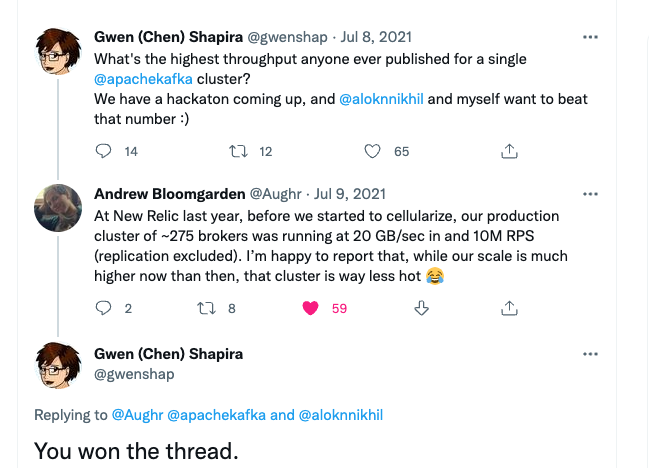
\includegraphics[keepaspectratio,width=\textwidth,height=0.8\textheight]{twitter.png}
  \end{center}
\end{frame}

\begin{frame}
  \frametitle{MSK regional bytes}

  \begin{center}
    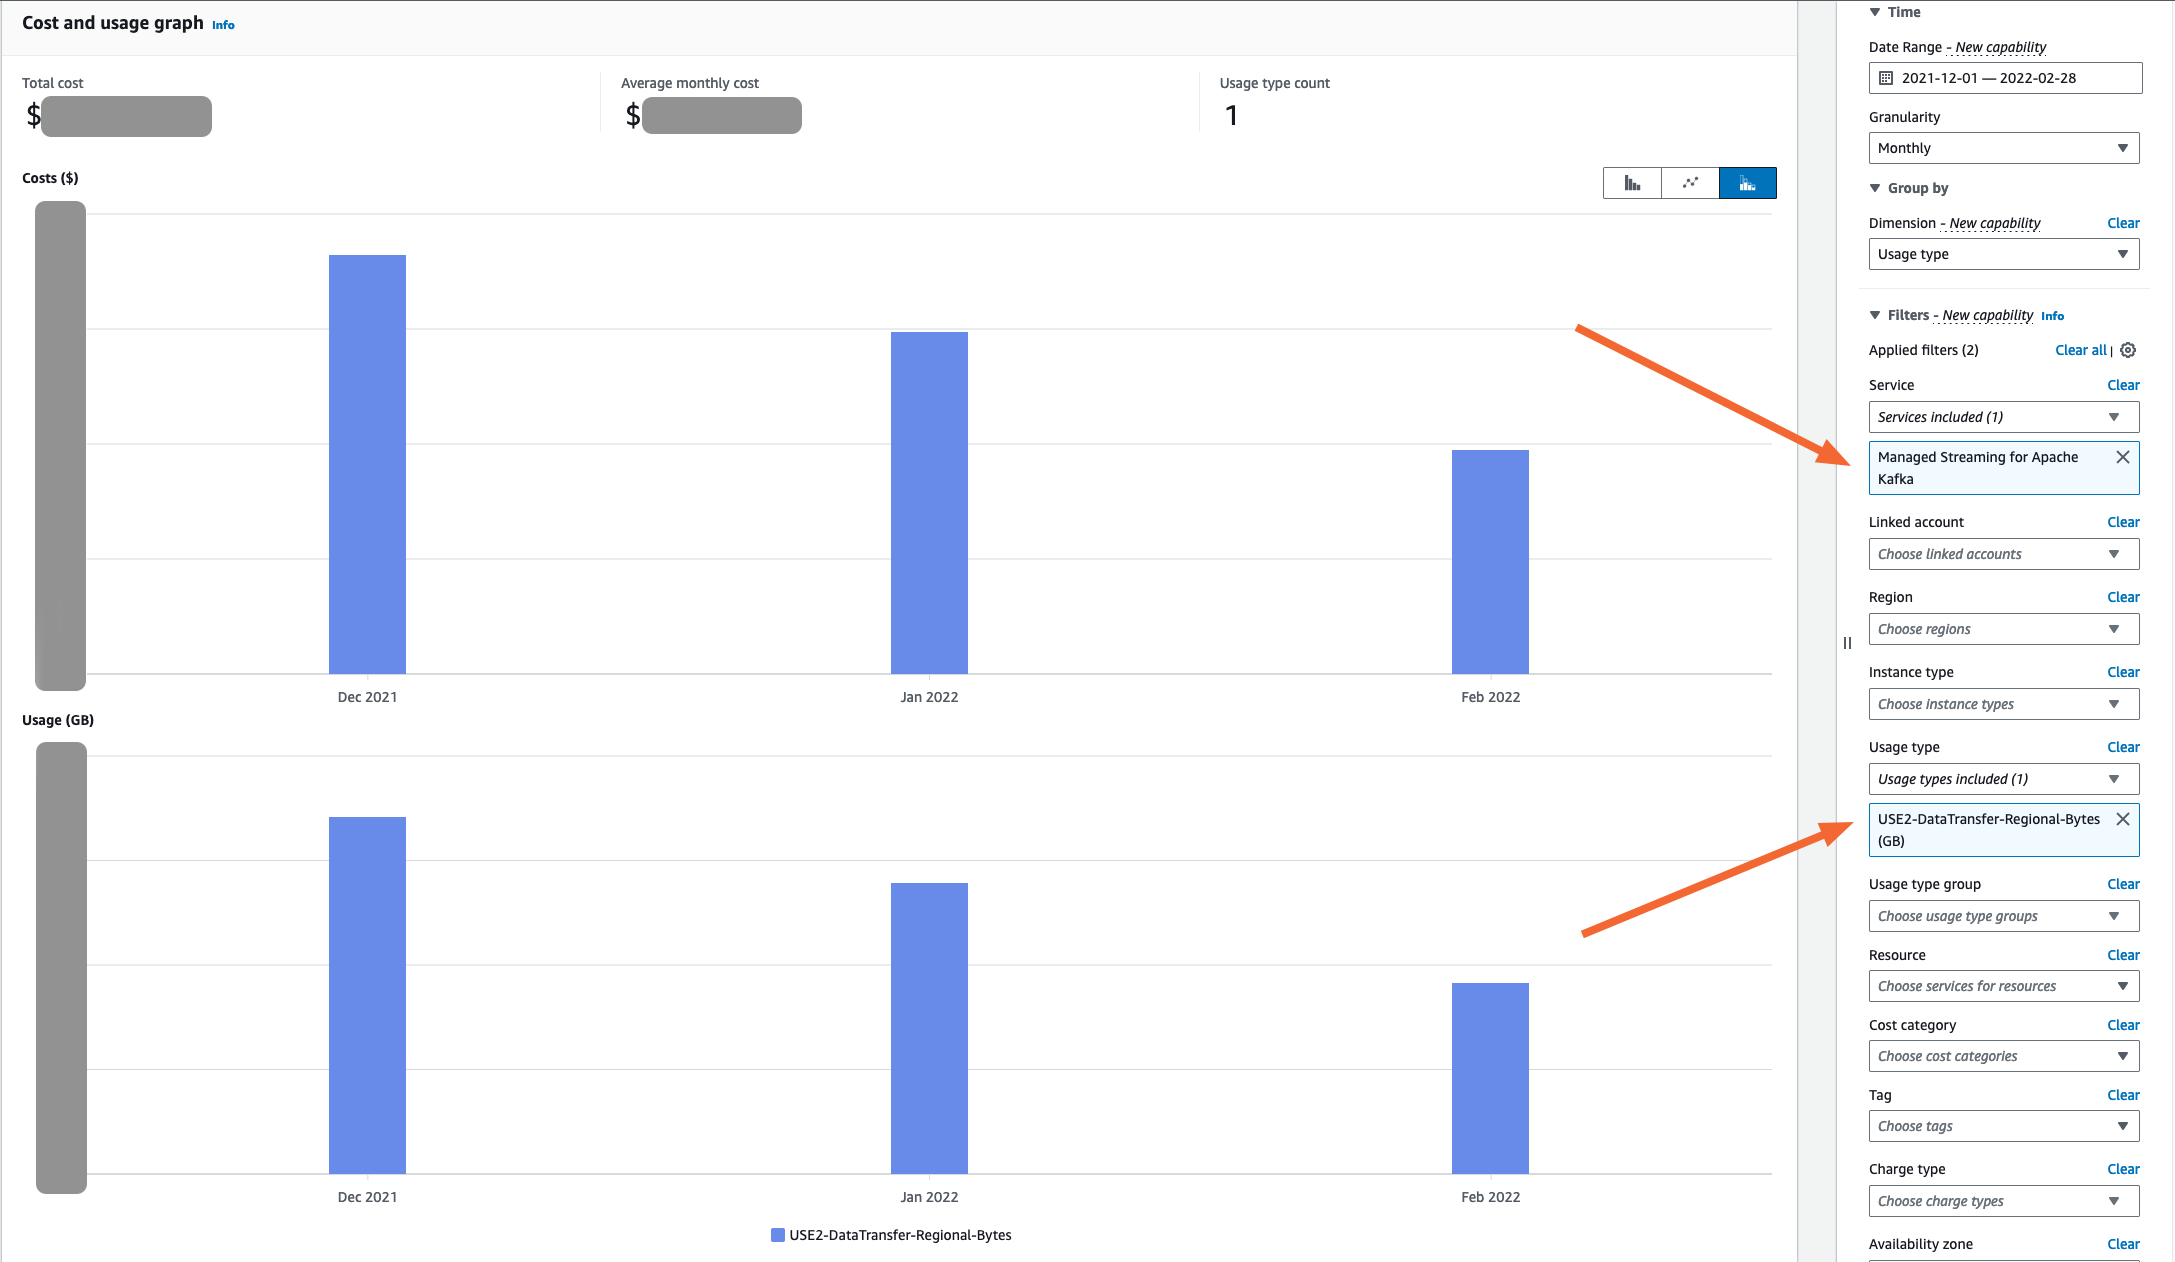
\includegraphics[keepaspectratio,width=\textwidth,height=0.8\textheight]{msk.png}
  \end{center}
\end{frame}

\begin{frame}
  \frametitle{EC2 regional bytes}

  \begin{center}
    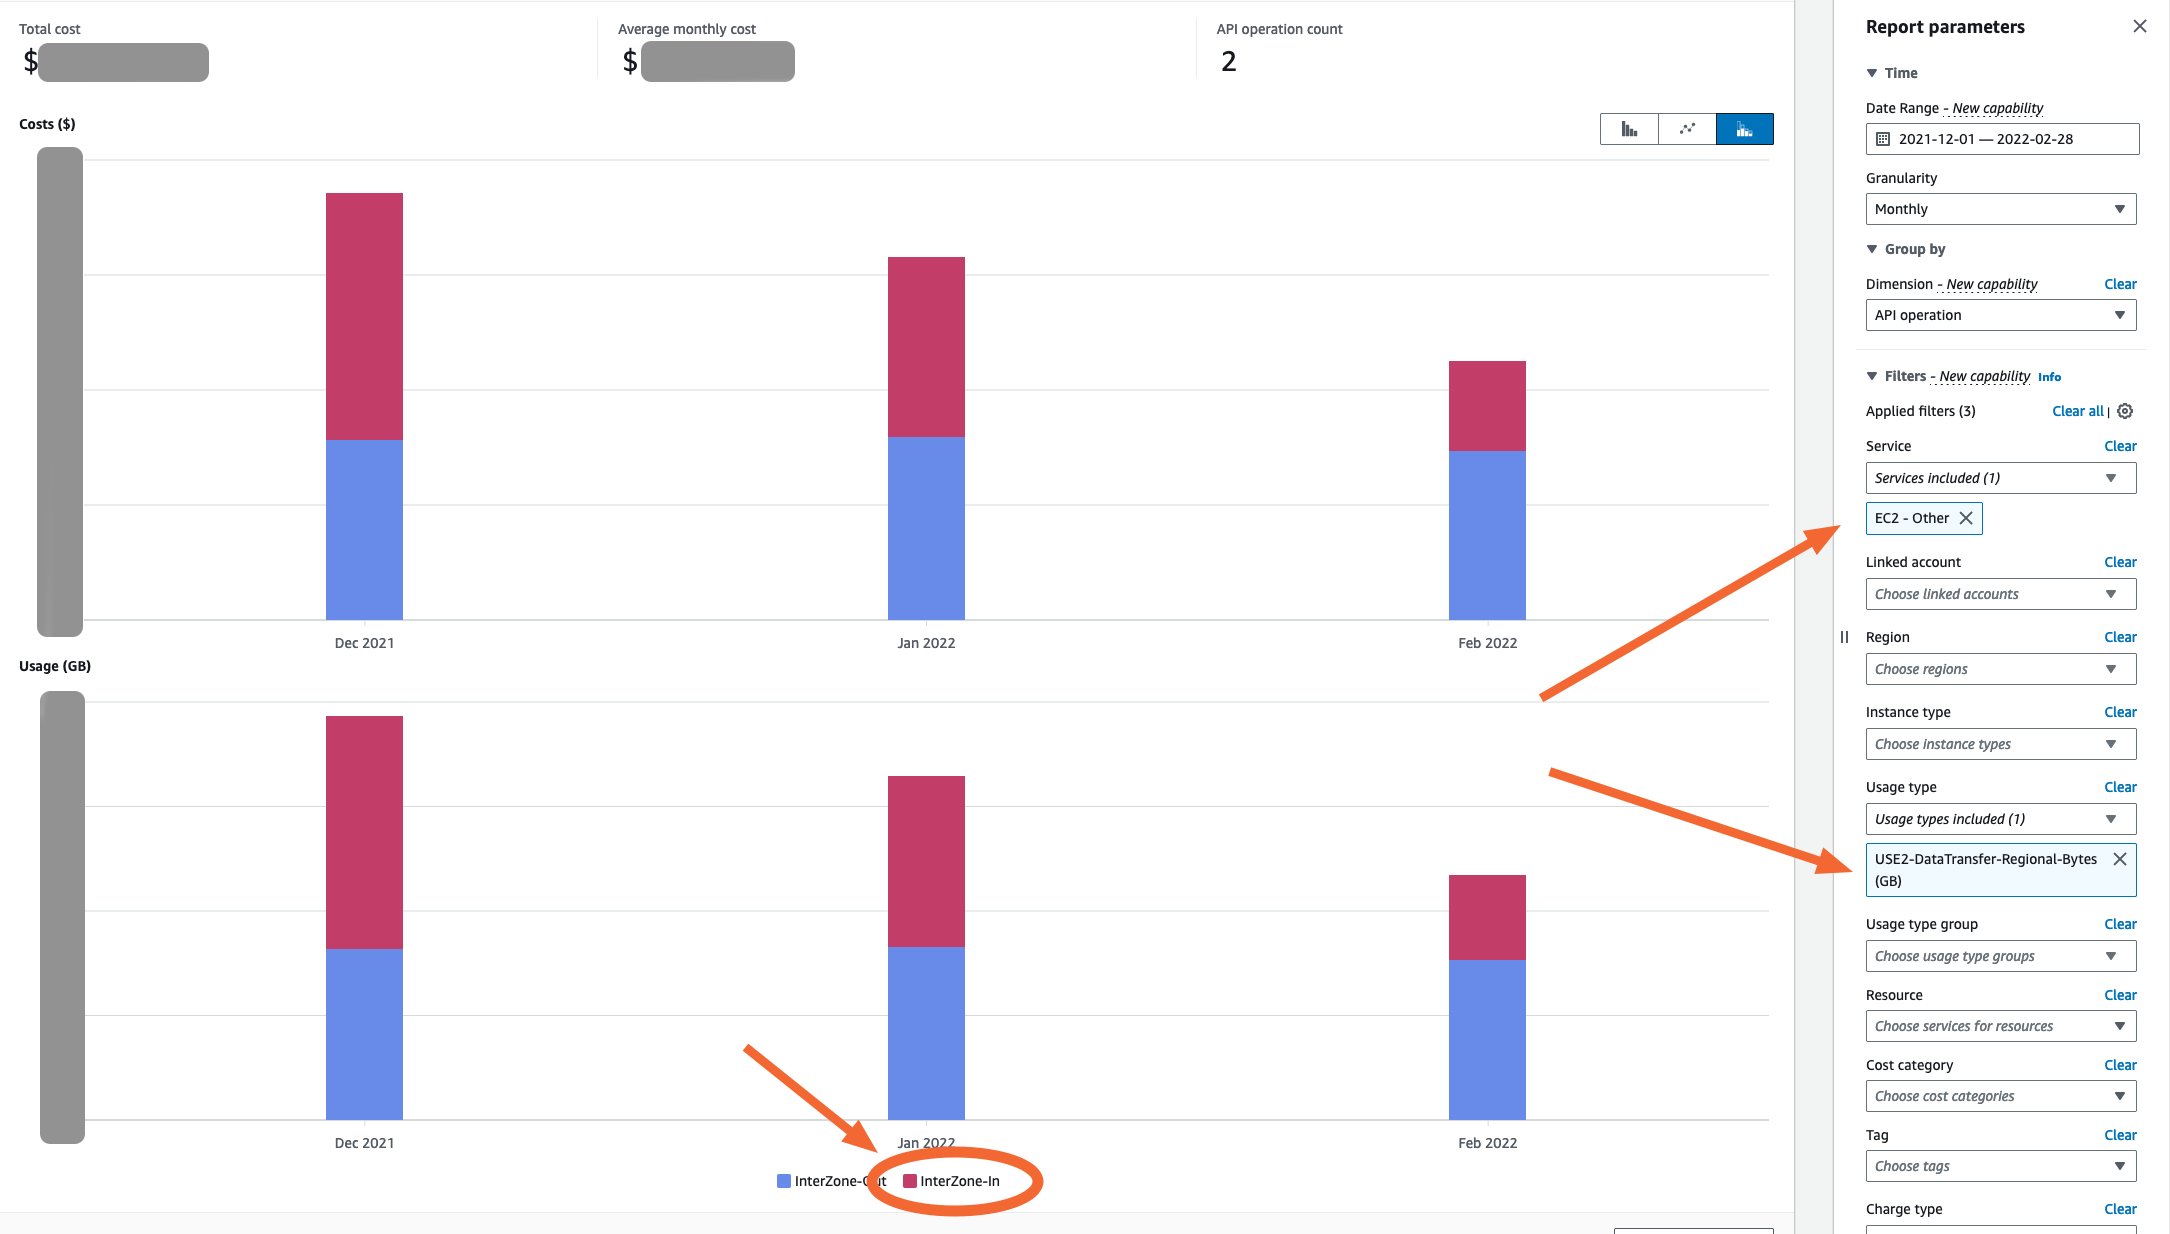
\includegraphics[keepaspectratio,width=\textwidth,height=0.8\textheight]{ec2.png}
  \end{center}
\end{frame}

\begin{frame}
  \frametitle{Overall regional bytes}

  \begin{center}
    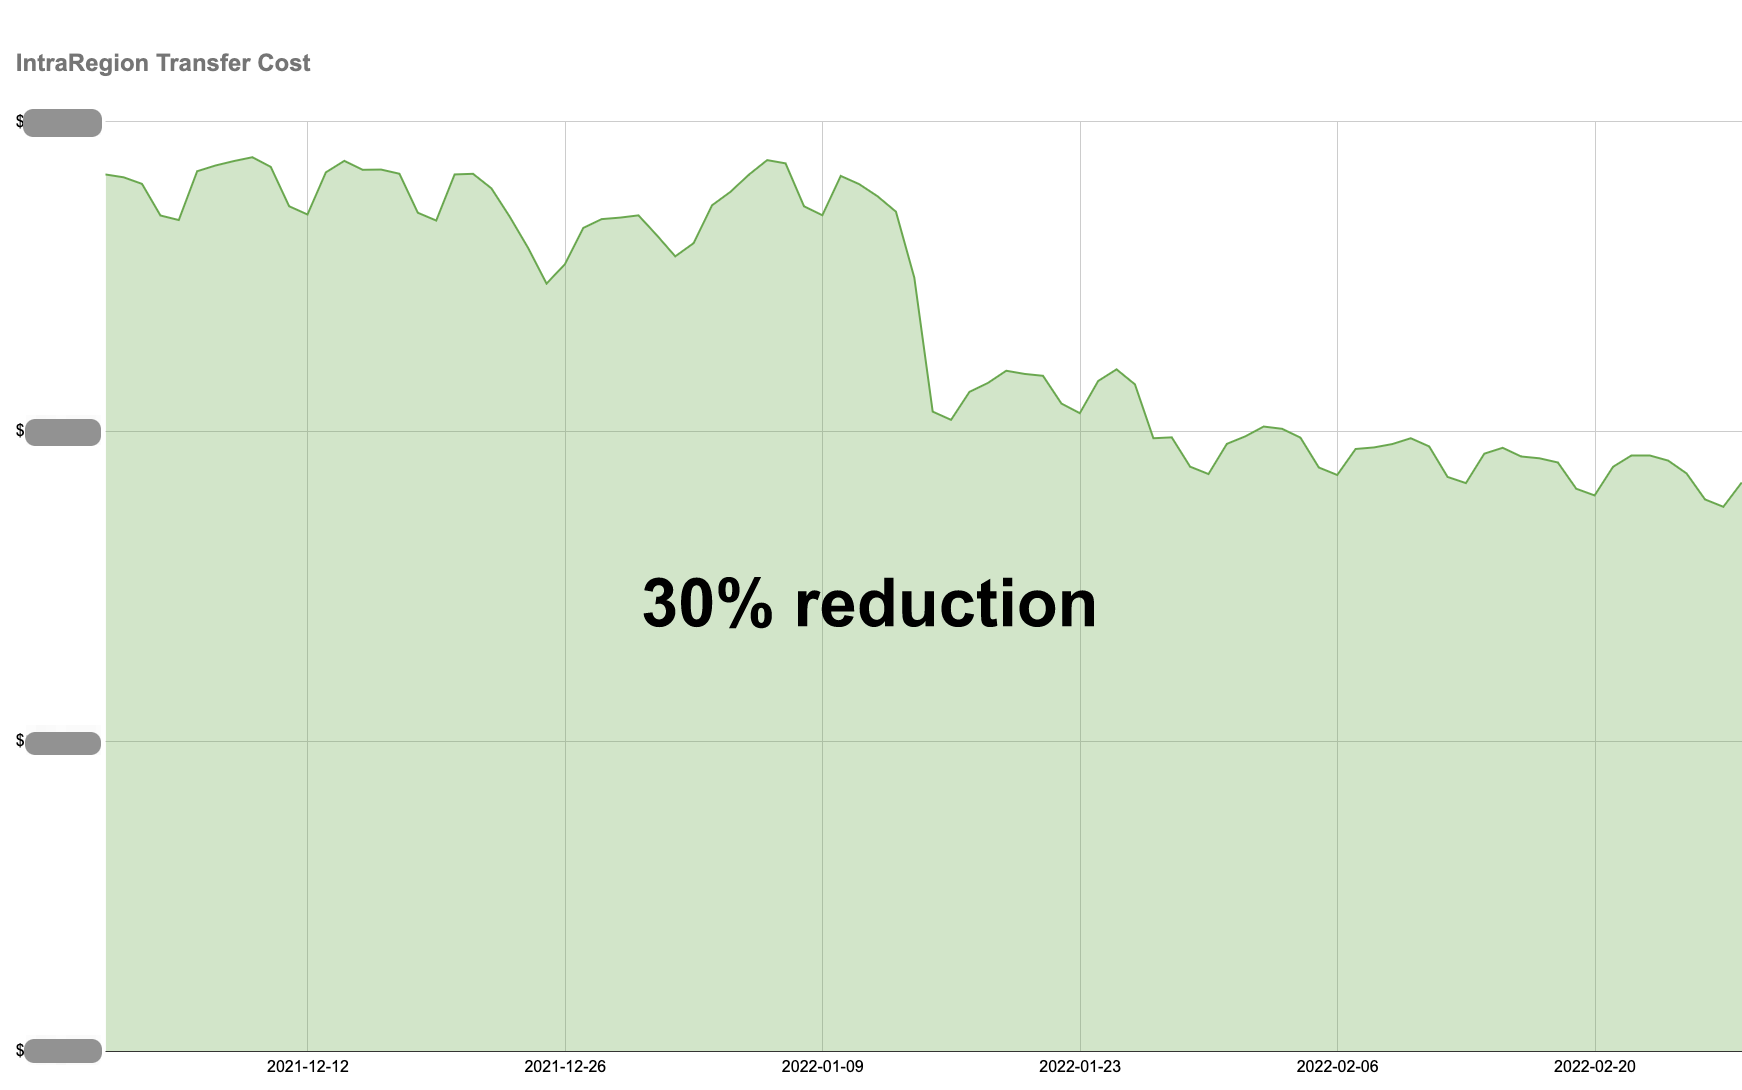
\includegraphics[keepaspectratio,width=\textwidth,height=0.8\textheight]{overall.png}
  \end{center}
\end{frame}

\subsection{Potential improvements}

\begin{frame}
  \frametitle{What about InterZone-out?}

  \begin{center}
    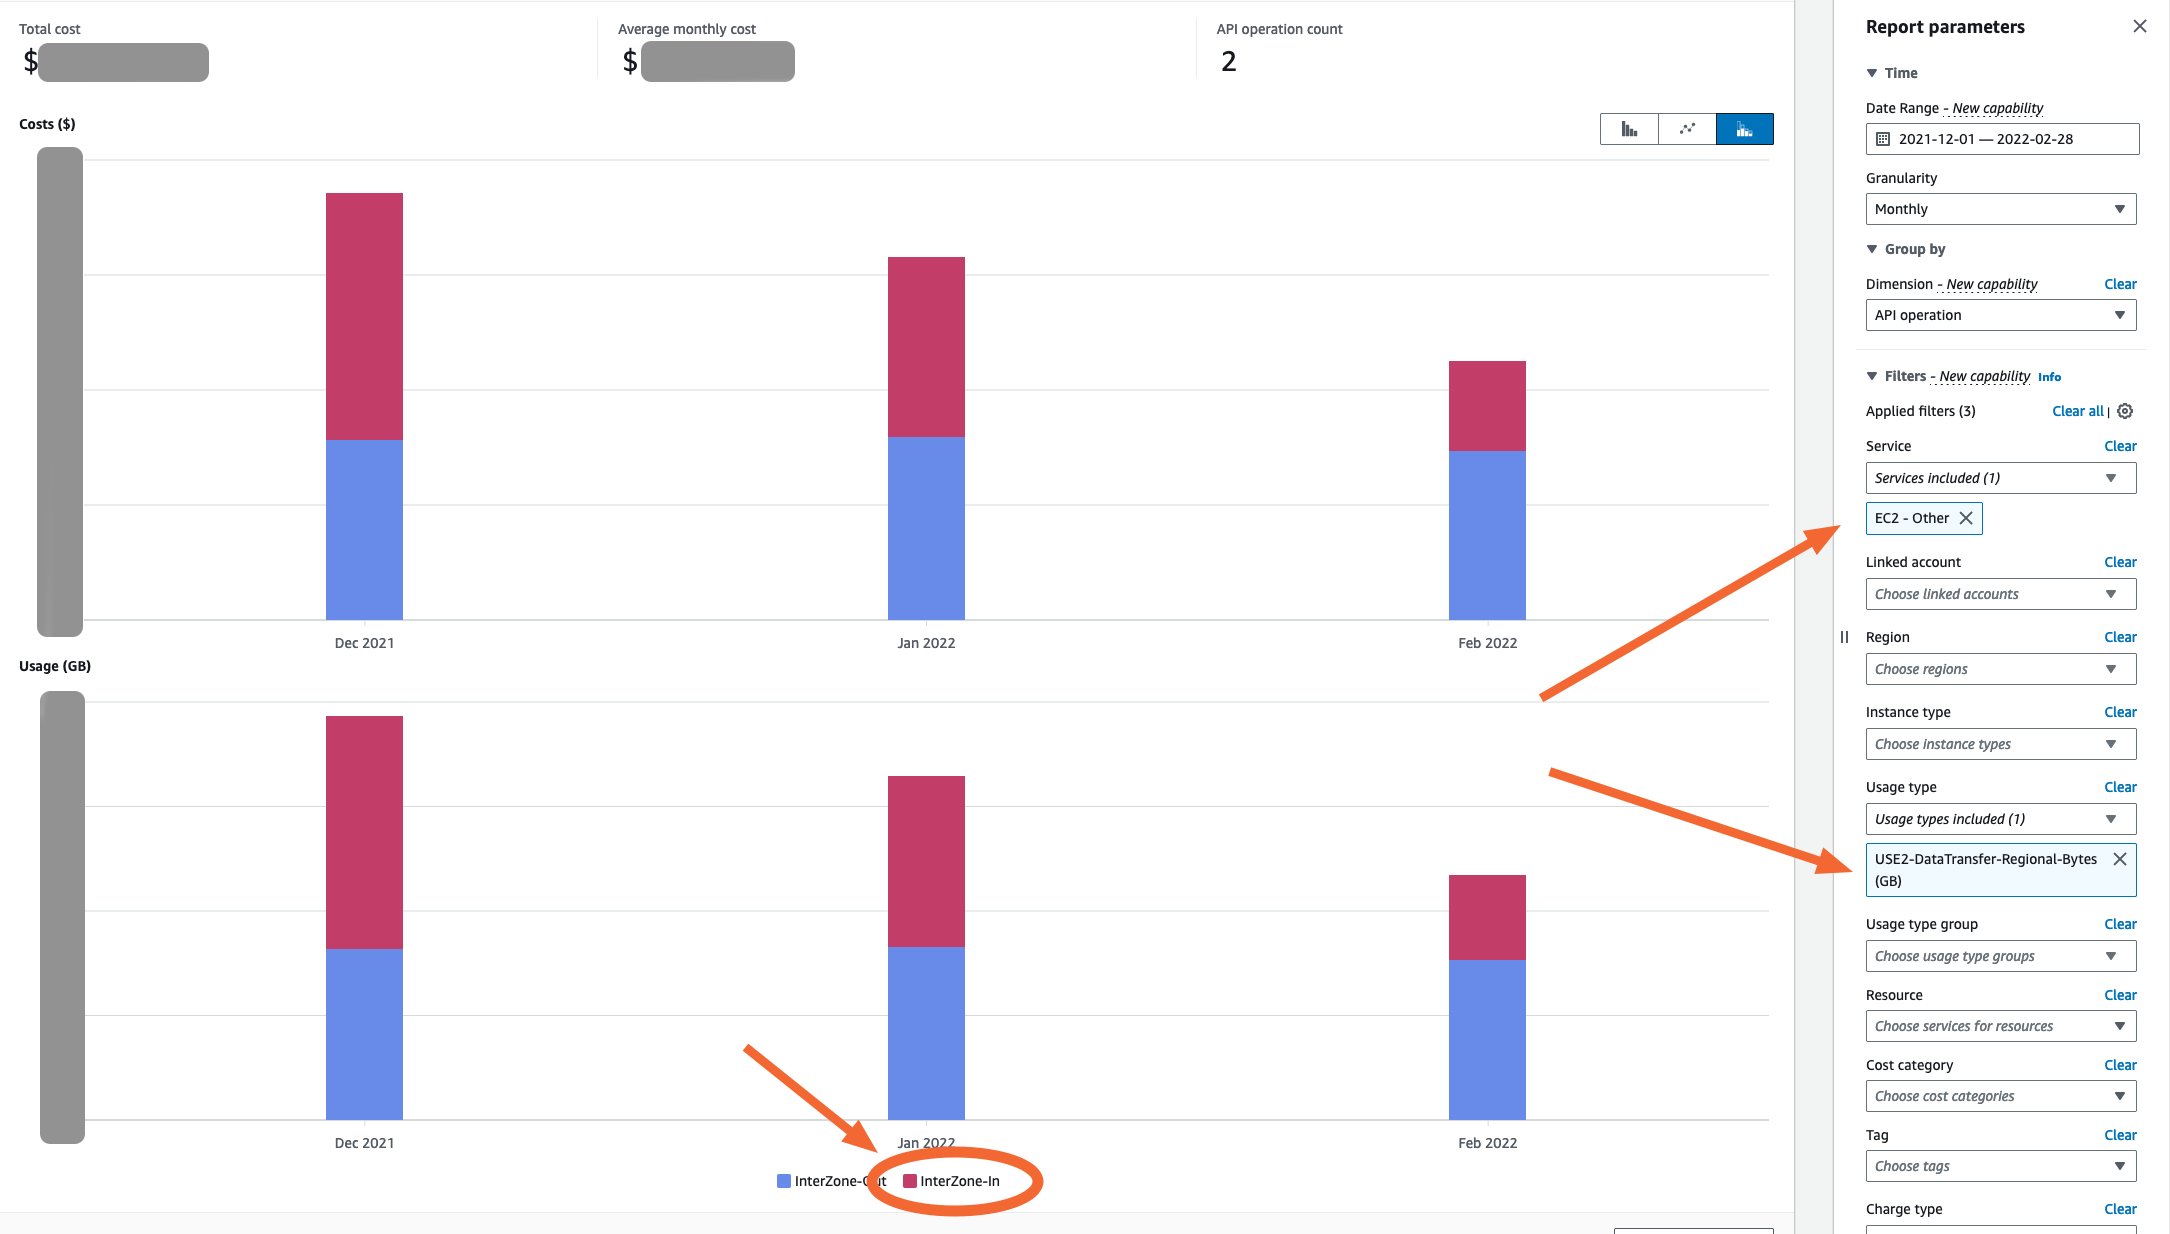
\includegraphics[keepaspectratio,width=\textwidth,height=0.8\textheight]{ec2.png}
  \end{center}
\end{frame}

\begin{frame}
  \frametitle{Rack-aware producing}

  \begin{itemize}
  \item some producers \alert{don't use keys} for partitioning
  \item idea: \alert{only pick} from partitions led by brokers in the \alert{producer's rack}
  \item implemented as a \alert{custom partitioner}
  \end{itemize}
\end{frame}

\begin{frame}
  \frametitle{Rack-aware partitioner}

  \begin{beamercolorbox}[sep=1em]{code}
    \usebeamerfont{code}
    \include{RackAwarePartitioner}
  \end{beamercolorbox}
\end{frame}

\begin{frame}
  \frametitle{Not as good a rack-aware consuming}

  \begin{itemize}
  \item only works for \alert{randomly} partitioned topics
  \item needs producers to be \alert{uniformly} distributed among AZs
    \begin{itemize}
    \item risks creating hot partitions otherwise
    \end{itemize}
  \item does not use \alert{sticky partitioning}
    \begin{itemize}
    \item no access to the \texttt{BuiltInPartitioner}
    \item no access to broker load stats to emulate load-driven sticky partitioning
    \end{itemize}
  \end{itemize}
\end{frame}

\begin{frame}
  \frametitle{Still kind of works, though!}

  \begin{center}
    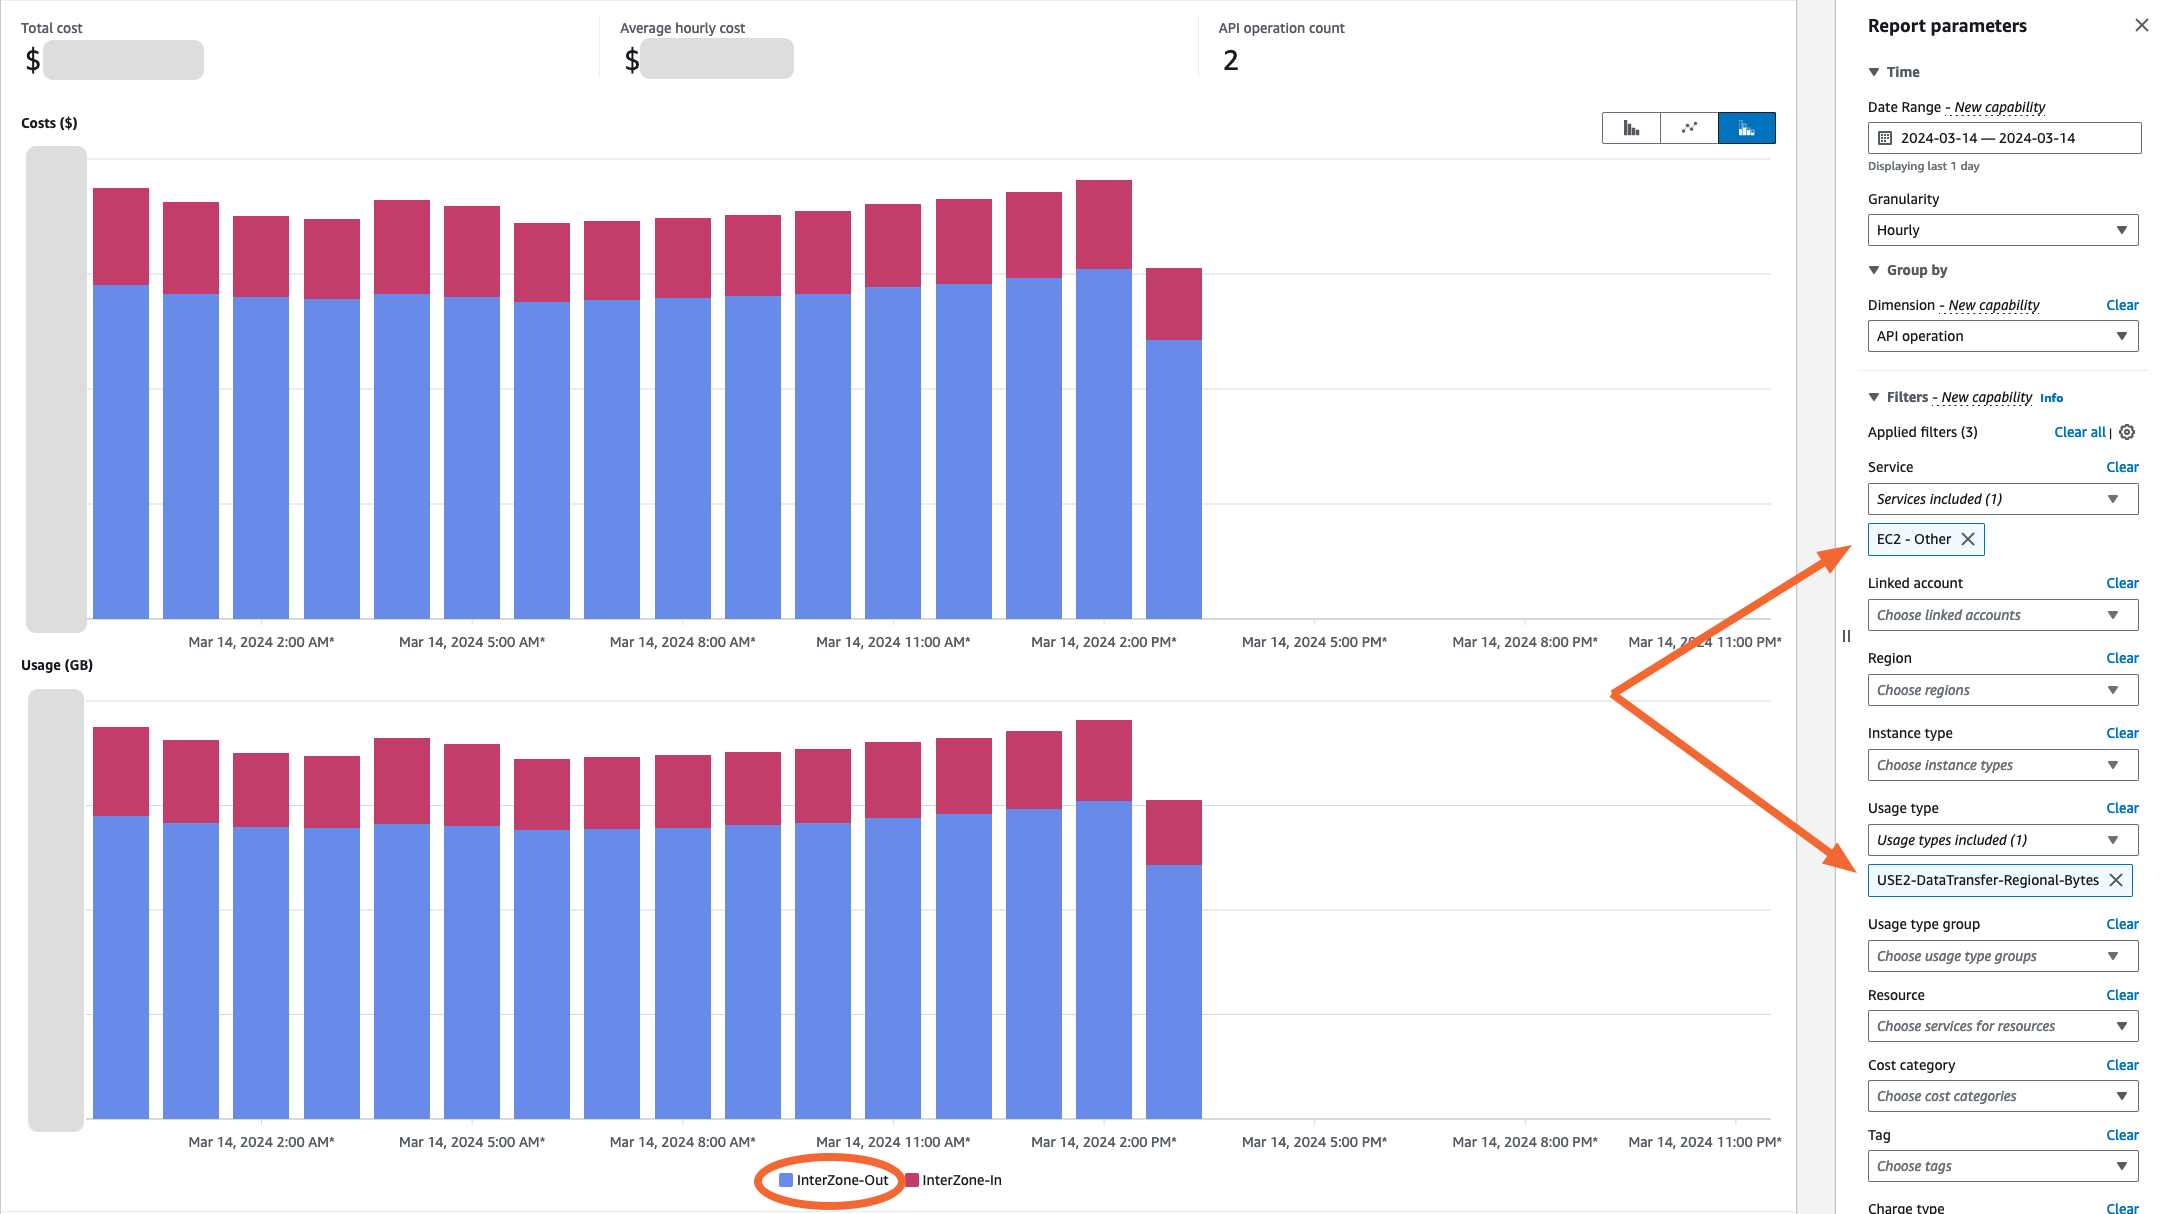
\includegraphics[keepaspectratio,width=\textwidth,height=0.8\textheight]{producer.png}
  \end{center}
\end{frame}

\subsection*{Questions}

\begin{frame}
\begin{beamercolorbox}[center]{note}
  \Huge Questions?
\end{beamercolorbox}
\end{frame}

\end{document}
